% \documentclass[a4paper,10pt]{article}
% % Wenn Sie eine andere Dokumentenklasse benutzen, kann sich das Layout verschieben 
% %({scrreprt} verursacht beispielsweise einen ungewollten Seitenumbruch).
% % Sie können in diesem Fall versuchen, die Abstände (\vspace, siehe unten) anzupassen 
% % oder Sie compilieren das Titelblatt einzeln mit der Dokumentenklasse "`article"'.
% \usepackage{graphicx}
% \usepackage{float}
% \usepackage[T1]{fontenc}
% 
% \begin{document}
\thispagestyle{empty}

\hspace{20cm}
\vspace{-2cm}

\begin{center}
  %\vspace{0.5 cm}
  \huge{\bf Titel der Arbeit} \\ % Hier fuegen Sie den Titel Ihrer Arbeit ein.
  \vspace{1cm}
  \LARGE  Bachelorarbeit \\ % Geben Sie anstelle der Punkte an, ob es sich um eine
                % Diplomarbeit, eine Masterarbeit oder eine Bachelorarbeit handelt.
  \vspace{0.3cm}
  \large Abschlussarbeit zur Erlangung des akademischen Grades Bachelor of Science (B.Sc.) \\
an der Hochschule für Technik und Wirtschaft Berlin \\ % Bitte tragen Sie hier anstelle der Punkte ein:
         % Diplominformatiker(in),
         % Bachelor of Arts (B. A.),
         % Bachelor of Science (B. Sc.),
         % Master of Education (M. Ed.) oder
         % Master of Science (M. Sc.).
  \vspace{1cm}
  {\large
    %\bf{
      \scshape
      %Humboldt-Universit\"at zu Berlin \\
      Fachbereich Informatik, Kommunikation und Wirtschaft \\
      Studiengang Informatik und Wirtschaft\\
    %}
  } 
  % \normalfont
\end{center}
\vspace {0.5 cm}% gegebenenfalls kleiner, falls der Titel der Arbeit sehr lang sein sollte
%{3.2 cm} bei Verwendung von scrreprt, gegebenenfalls kleiner, falls der Titel der Arbeit sehr lang sein sollte
{\large
  \begin{tabular}{llll}
    eingereicht von:    & Vorname Name && \\ % Bitte Vor- und Nachnamen anstelle der Punkte eintragen.
    Matrikelnummer:     & 123456          &&
    %geboren am:         & 02.11.1980 && \\
    %in:                 & Berlin && \\
    \cr&\\
    Gutachter/Innen: & Prof. Dr. xy && \\
		      & yz && \\% Bitte Namen der Gutachter(innen) anstelle der Punkte eintragen
				 % bei zwei männlichen Gutachtern kann das (innen) weggestrichen werden
    &&&\\
    eingereicht am:     & \dots\dots  \hspace{3cm} verteidigt am: & \dots\dots \\ % Bitte lassen Sie
                                    % diese beiden Felder leer.
                                    % Loeschen Sie ggf. das letzte Feld, wenn
                                    % Sie Ihre Arbeit laut Pruefungsordnung nicht
                                    % verteidigen muessen.
  \end{tabular}
}
\vspace{0.3 cm}
\begin{figure}[H] 
  \begin{center}
    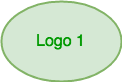
\includegraphics[width=4 cm]{img/logo1}
    \hspace{2cm}
    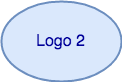
\includegraphics[width=4 cm]{img/logo2}
  \end{center}
\end{figure}
% \end{document}


%%%%%% ALTES TITELBLATT:
% %%%%%%%% TITLE %%%%%%%%%%%%%%%%%%%%%%%%%%%%%%%%%%%%%%%%%%%%%%%%%%%%%%%%%%%%%%%%%
% \begin{minipage}{17cm}
% %\begin{titlepage}
% \thispagestyle{empty}
% \begin{center} 
% \LARGE{ \vspace{2ex} Diplomarbeit}\\[4ex] 
% \huge{Rankingverfahren für Dokumentensuche basierend auf Ontologie-Relationen} \\[4ex]
% \large{ eingereicht von: Benjamin Großmann}\\[4ex]
% \large{ Berlin, den \dategerman \today}\\[8ex]
% 
%   \normalsize{
%   \psfig{figure=Bilder/husiegel_sw_klein,height=16ex}\\
%   Mathematisch-Naturwissenschaftliche \\Fakult\"at II\\Institut f\"ur Informatik\\[4ex]
%   }
%   \large{Betreuer:\\[1ex]
% %	Dr. Christian Herta, neofonie GmbH \\ [1ex]
% %	Prof. Dr. Hans-Dieter Burkhard, Humboldt-Universität zu Berlin, Lehrstuhl Künstliche Intelligenz
% 	}
% 	
% \end{center}
% \end{minipage}
%\newpage
